% Presentación final — Proyecto 1 · Planifica
% Compilar: cd presentacion && tectonic planifica_presentacion.tex
\documentclass[aspectratio=169,11pt]{beamer}
\usepackage[spanish,es-tabla]{babel}
\usepackage{lmodern}
\usepackage{booktabs}
\usepackage{graphicx}
\usepackage{tabularx}
\usepackage{array}

\graphicspath{{figures/}{../informe_latex/figures/}}

\definecolor{ink}{HTML}{13263A}
\definecolor{teal}{HTML}{0F766E}
\definecolor{coral}{HTML}{D95B43}
\definecolor{slate}{HTML}{52606D}
\definecolor{mist}{HTML}{EEF4F5}

\setbeamertemplate{navigation symbols}{}
\setbeamercolor{background canvas}{bg=white}
\setbeamercolor{frametitle}{bg=ink,fg=white}
\setbeamercolor{title}{fg=ink}
\setbeamercolor{block title}{bg=teal,fg=white}
\setbeamercolor{block body}{bg=mist,fg=ink}
\setbeamercolor{block title alerted}{bg=coral,fg=white}
\setbeamercolor{block body alerted}{bg=mist,fg=ink}
\setbeamerfont{frametitle}{series=\bfseries,size=\large}
\setbeamerfont{block title}{series=\bfseries,size=\normalsize}

\newcommand{\statcard}[3]{%
  \begin{beamercolorbox}[center,sep=0.20cm,rounded=true]{#2}%
    {\Large\bfseries #3}\par\vspace{0.02em}{\footnotesize #1}%
  \end{beamercolorbox}%
}

\setbeamertemplate{footline}{%
  \leavevmode%
  \hbox{%
    \begin{beamercolorbox}[wd=.75\paperwidth,ht=2.4mm,dp=1.6mm,leftskip=2mm]{author in head/foot}%
      \color{slate}\scriptsize Proyecto 1 · Planificación y Toma de Decisiones en IA
    \end{beamercolorbox}%
    \begin{beamercolorbox}[wd=.25\paperwidth,ht=2.4mm,dp=1.6mm,rightskip=2mm]{page number in head/foot}%
      \hfill\color{slate}\scriptsize\insertframenumber\,/\,\inserttotalframenumber
    \end{beamercolorbox}}%
}
\setbeamercolor{author in head/foot}{bg=white}
\setbeamercolor{page number in head/foot}{bg=white}

\title{Sistema inteligente adaptativo para detección de fraude}
\subtitle{IEEE-CIS Fraud Detection · datos no estacionarios}
\author{Edgar Chambilla}
\date{Septiembre 2026}

\begin{document}

% 1 --------------------------------------------------------------------------
\begin{frame}
  \vspace{0.3em}
  {\scriptsize\color{coral}\bfseries PROYECTO 1}\\[0.2em]
  {\color{ink}\Huge\bfseries Sistema inteligente adaptativo\\[0.15em] para detección de fraude}\\[0.45em]
  {\color{slate}\large IEEE-CIS Fraud Detection · datos no estacionarios}\\[0.15em]
  {\color{slate}Validación temporal, contexto de entidad y monitoreo operativo}

  \vspace{0.9em}
  \begin{center}
    \begin{tabular}{ccc}
      {\color{teal}\bfseries DATOS} & {\color{teal}\bfseries MODELO} & {\color{teal}\bfseries ADAPTACIÓN}\\
      orden temporal & score de fraude & PSI + ventanas\\
    \end{tabular}
    \vspace{0.5em}

    \colorbox{mist}{\parbox{0.78\textwidth}{\centering
      \color{ink}\bfseries 590\,540 transacciones \quad · \quad +0,0116 AUC con magic UID \quad · \quad 4 ventanas temporales}}
  \end{center}
  \vfill
  {\color{slate}Edgar Chambilla · Septiembre 2026}
\end{frame}

% 2 --------------------------------------------------------------------------
\begin{frame}{Fraude no estacionario: validar hacia el futuro}
  \framesubtitle{El test oficial ocurre después del train; un split aleatorio no representa ese escenario}
  \begin{columns}[T]
    \begin{column}{0.34\textwidth}
      \statcard{transacciones · fraude 1:27}{mist}{\color{ink}590\,540 \;·\; \color{coral}3,50\%}
      \vspace{0.35em}
      \begin{alertblock}{Riesgo metodológico}
        \small El KFold aleatorio mezcla pasado y futuro e infla la estimación del AUC.
      \end{alertblock}
      \begin{block}{Pregunta del sistema}
        \small ¿Cuánto histórico debe recordar el modelo para decidir en el siguiente bloque?
      \end{block}
    \end{column}
    \begin{column}{0.64\textwidth}
      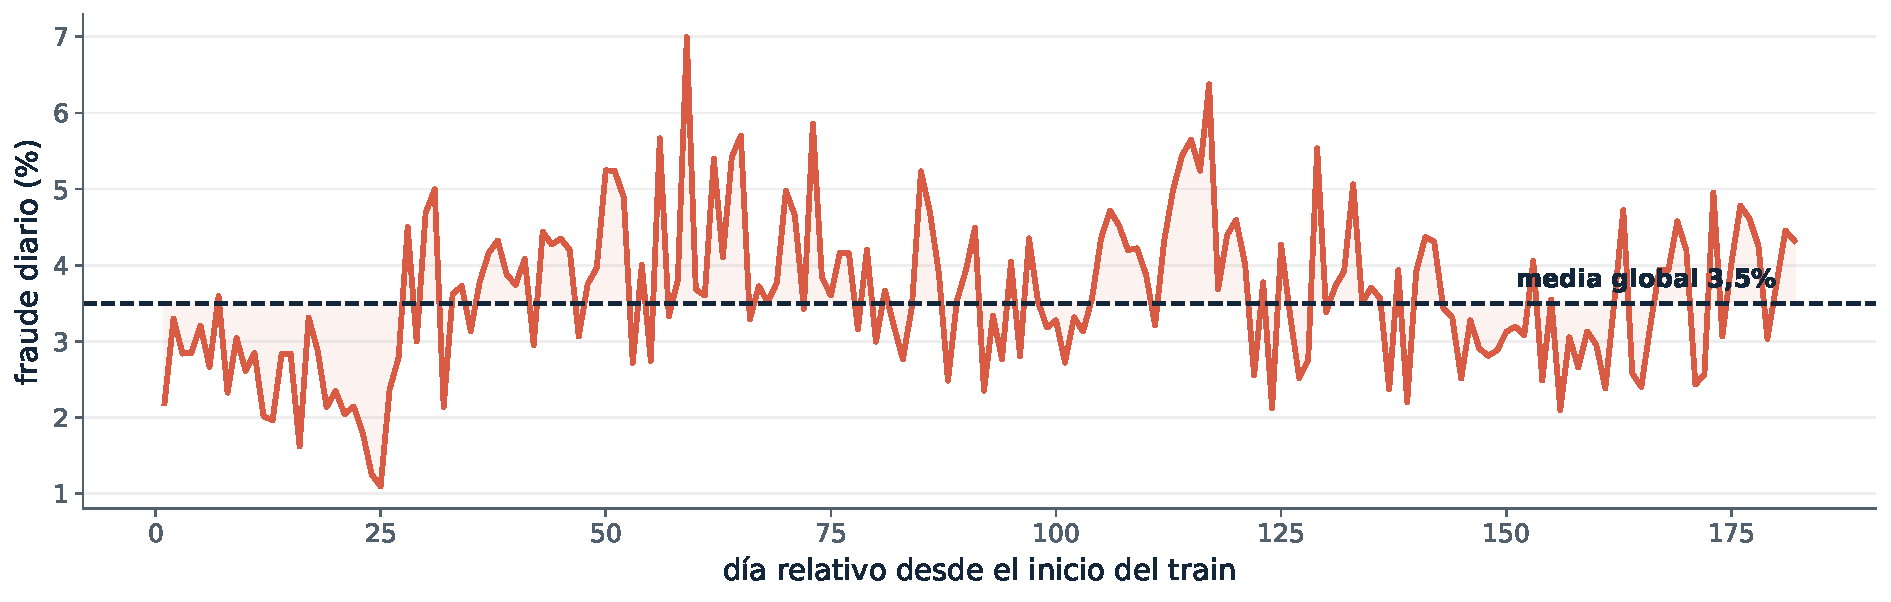
\includegraphics[width=\textwidth]{fraude_temporal.pdf}
      \vspace{0.2em}

      {\small\color{slate}La tasa diaria oscila alrededor de 3,5\% y presenta picos temporales: el rendimiento debe medirse por bloques futuros.}
    \end{column}
  \end{columns}
\end{frame}

% 3 --------------------------------------------------------------------------
\begin{frame}{La mejora dominante está en la representación}
  \framesubtitle{El hardware acelera; reconstruir contexto de cliente eleva el AUC}
  \begin{columns}[T]
    \begin{column}{0.27\textwidth}
      \statcard{mejor AUC local}{mist}{\color{teal}0,9479}
      \vspace{0.25em}
      \statcard{ganancia magic UID}{mist}{\color{teal}+0,0104}
      \vspace{0.25em}
      \statcard{aceleración GPU}{mist}{\color{ink}4,4×}
      \vspace{0.4em}
      {\small\color{slate}La GPU reduce tiempo; la ingeniería de entidad cambia el nivel de AUC con el mismo XGBoost d12.}
    \end{column}
    \begin{column}{0.71\textwidth}
      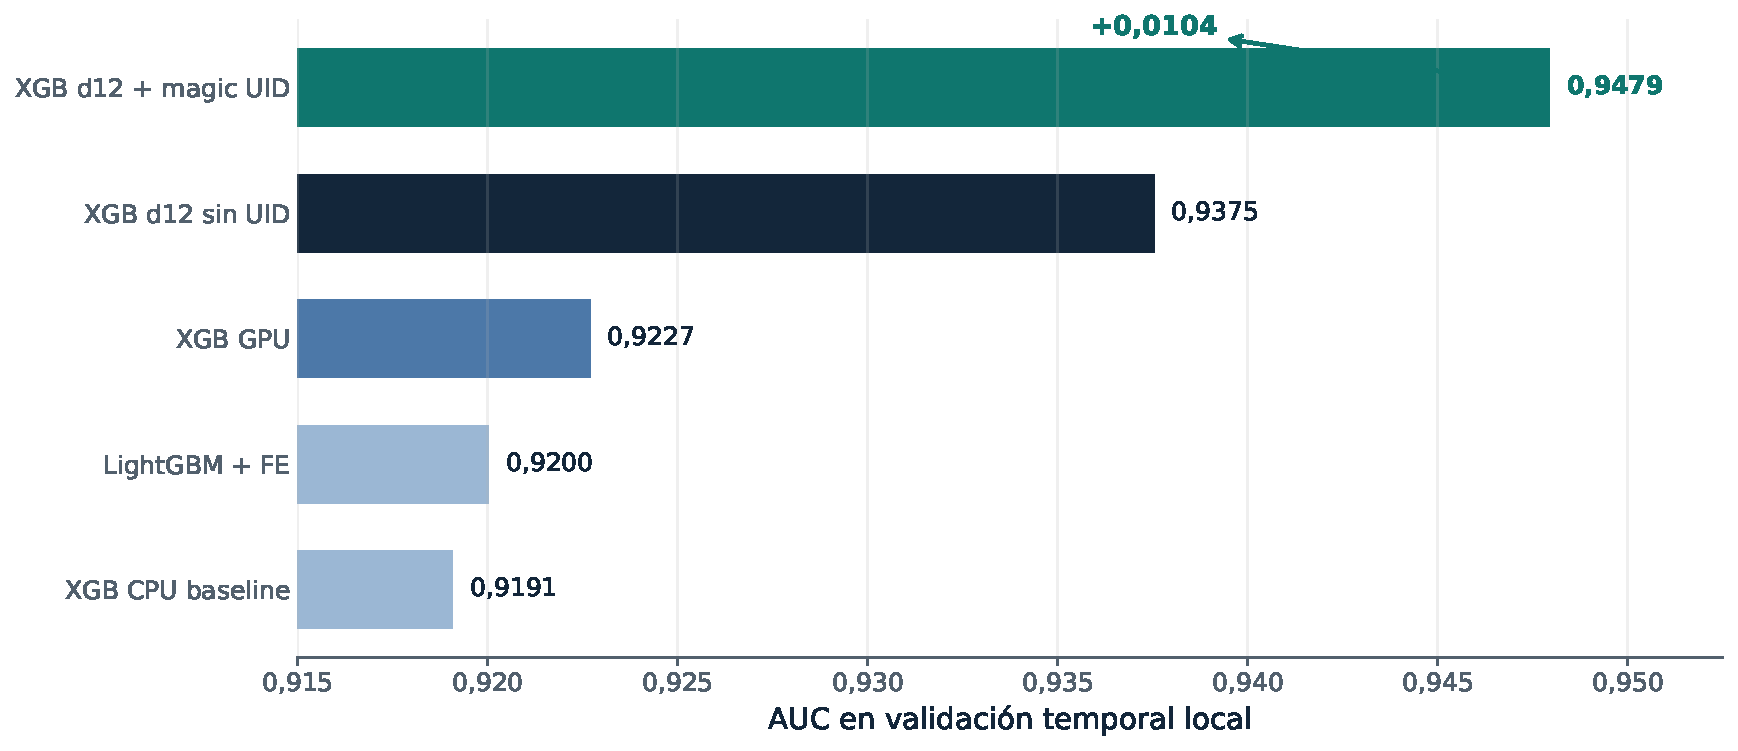
\includegraphics[width=\textwidth]{benchmark_auc.pdf}
    \end{column}
  \end{columns}
\end{frame}

% 4 --------------------------------------------------------------------------
\begin{frame}{Ablación propia: el magic UID aporta señal real}
  \framesubtitle{Notebook 05 · XGBoost d12 GPU · semilla 42 · mismo modelo y hardware}
  \begin{columns}[T]
    \begin{column}{0.29\textwidth}
      \begin{block}{Diseño experimental}
        \small
        \textbf{Sin UID:} 198 features\\[0.2em]
        \textbf{Con UID:} 245 features\\[0.2em]
        \textbf{Holdout:} 75/25 temporal\\[0.2em]
        \textbf{OOF:} GroupKFold mensual ×3
      \end{block}
      \begin{alertblock}{Ganancia pura}
        \small Solo cambia la representación: 
        \textbf{+0,0116} holdout y \textbf{+0,0162} OOF.
      \end{alertblock}
    \end{column}
    \begin{column}{0.69\textwidth}
      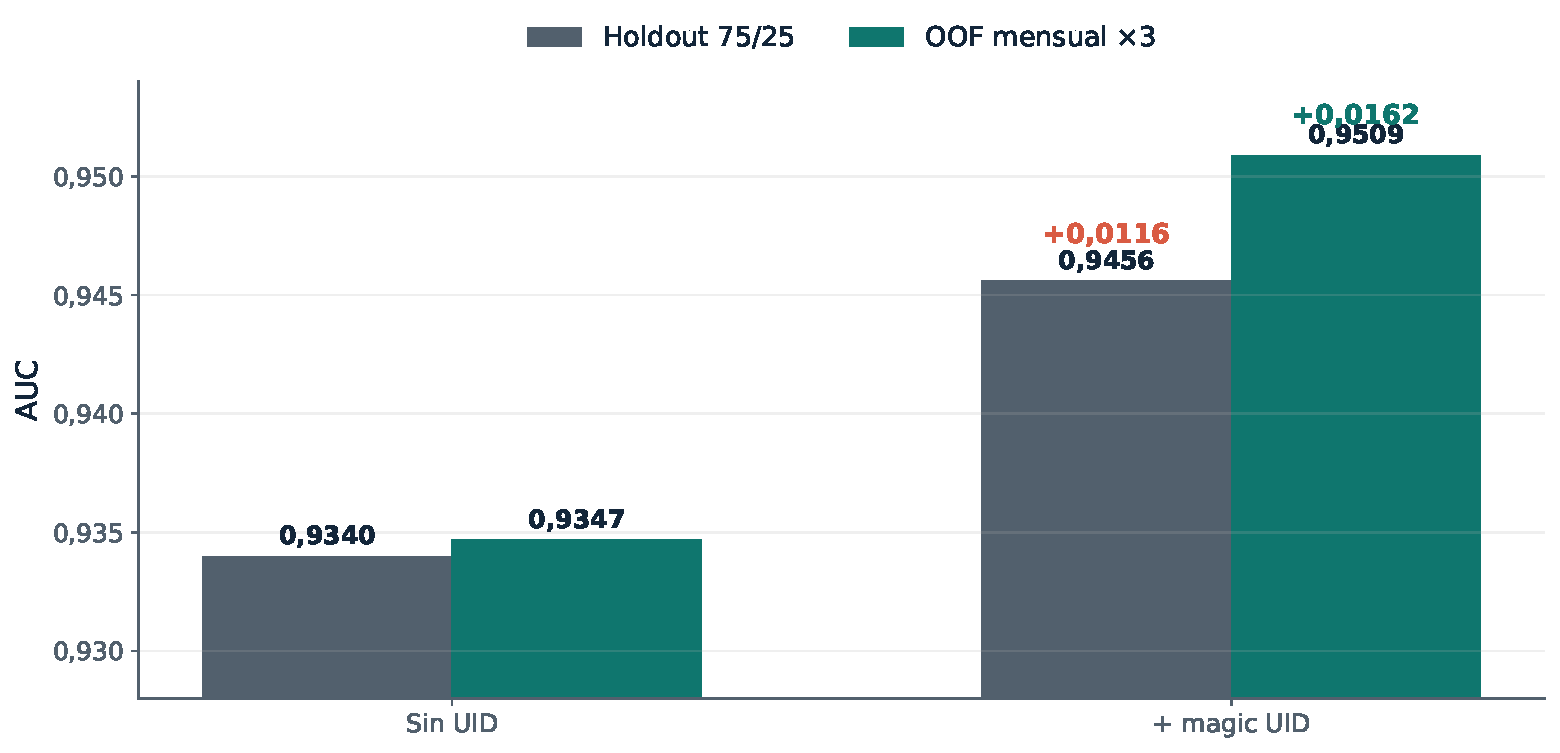
\includegraphics[width=\textwidth]{ablacion_uid.pdf}
    \end{column}
  \end{columns}
\end{frame}

% 5 --------------------------------------------------------------------------
\begin{frame}{El UID agrega contexto, pero nunca entra al modelo}
  \framesubtitle{Se reconstruye un pseudo-cliente y se conserva únicamente su historial agregado}
  \begin{center}
    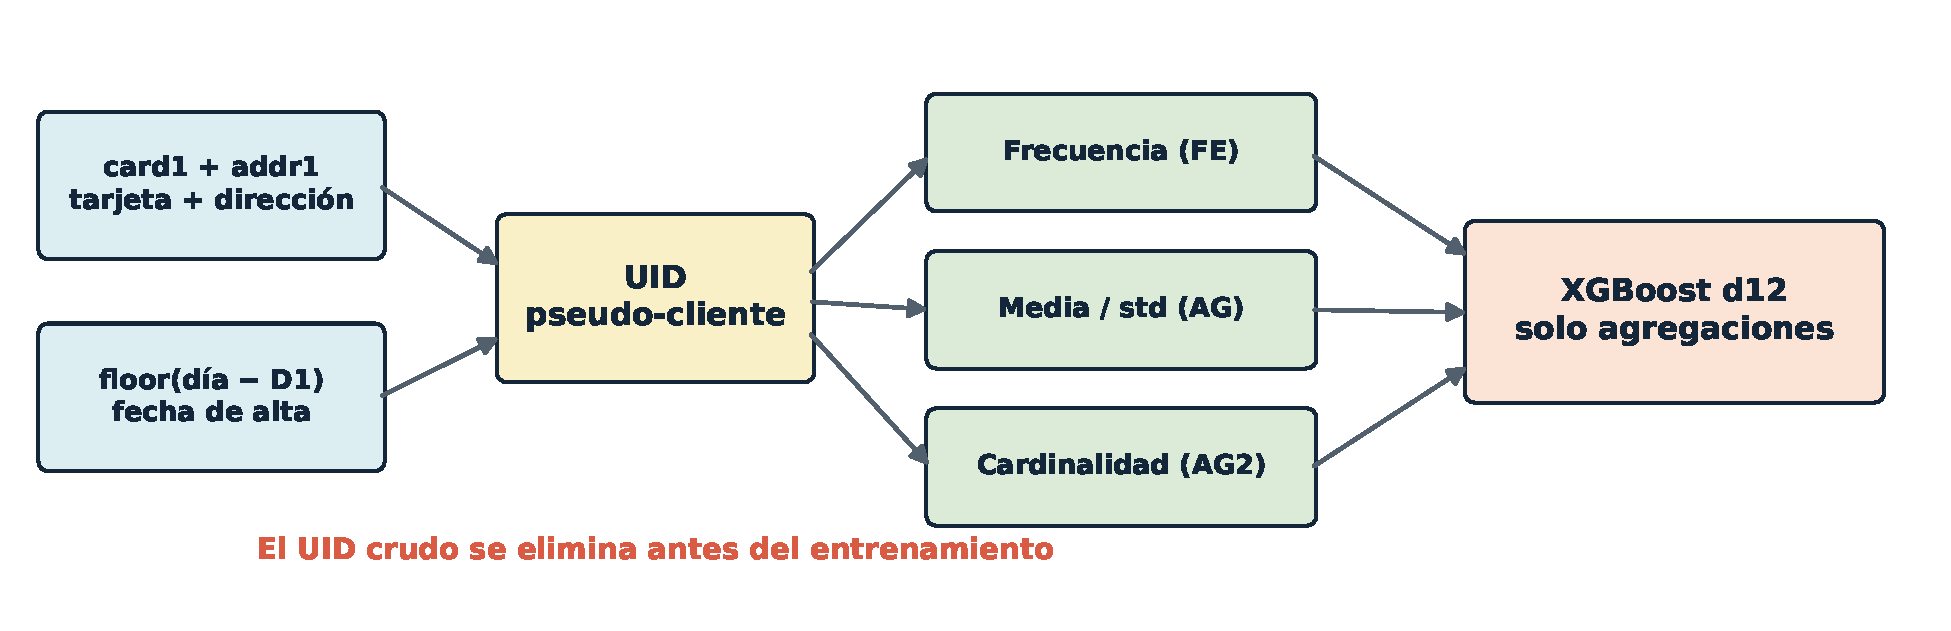
\includegraphics[width=0.96\textwidth]{uid_diagrama.pdf}
  \end{center}
  \vspace{-0.2em}
  \begin{columns}[T]
    \begin{column}{0.32\textwidth}
      \begin{block}{1 · Reconstruir}
        \small Tarjeta, dirección y antigüedad aproximan una entidad estable.
      \end{block}
    \end{column}
    \begin{column}{0.32\textwidth}
      \begin{block}{2 · Agregar}
        \small Frecuencia, media, dispersión y cardinalidad resumen su historial.
      \end{block}
    \end{column}
    \begin{column}{0.32\textwidth}
      \begin{block}{3 · Eliminar}
        \small El identificador crudo se descarta antes de entrenar XGBoost.
      \end{block}
    \end{column}
  \end{columns}
\end{frame}

% 6 --------------------------------------------------------------------------
\begin{frame}{De score a decisión: el umbral depende del costo}
  \framesubtitle{OOF notebook 04 · GroupKFold mensual ×6 · 590\,540 transacciones}
  \begin{center}
    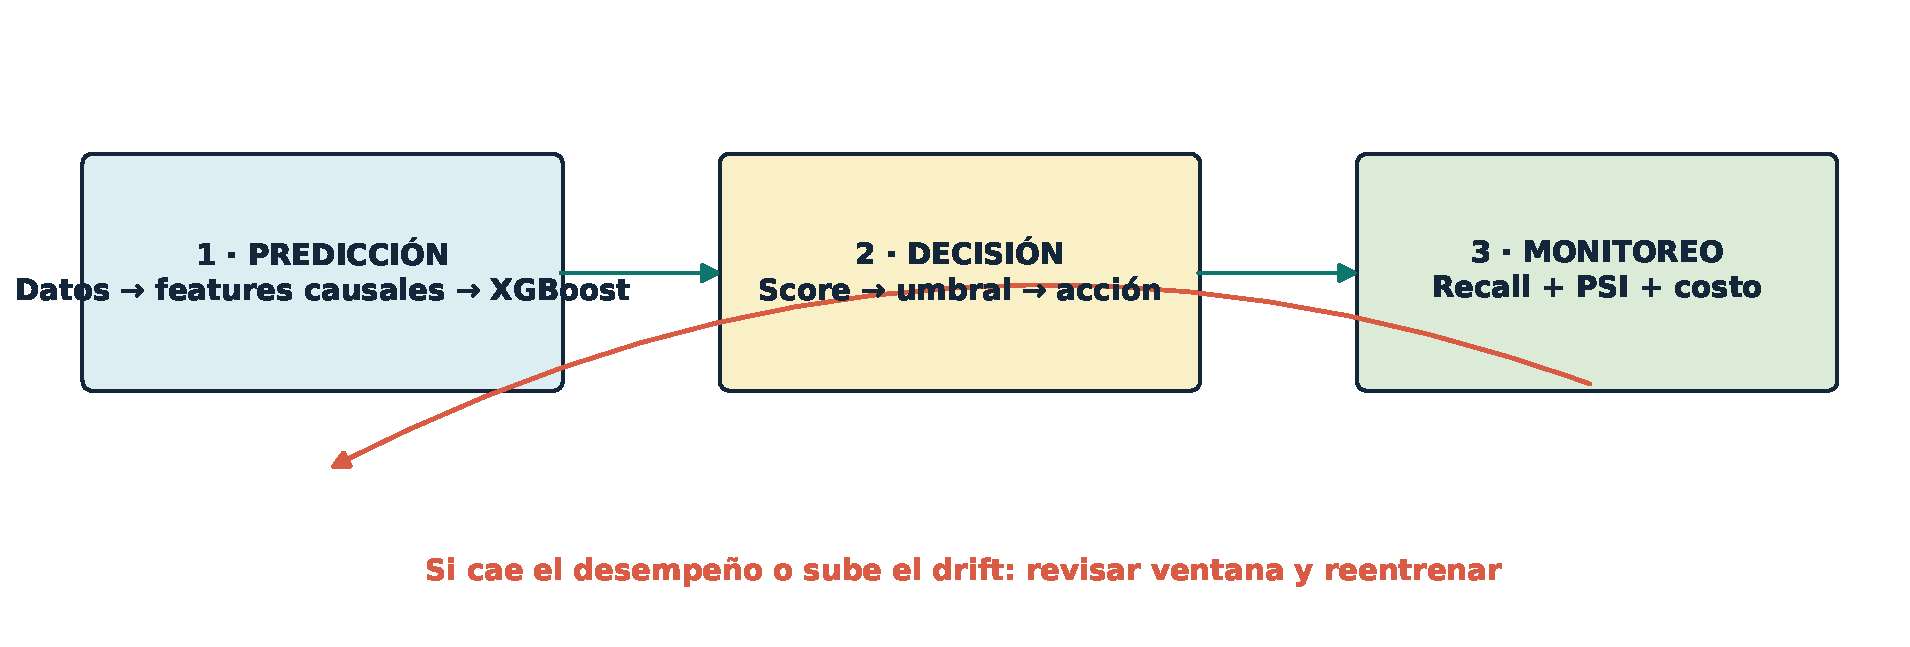
\includegraphics[width=0.82\textwidth]{pipeline_operativo.pdf}
  \end{center}
  \vspace{-0.35em}
  \begin{columns}[T]
    \begin{column}{0.55\textwidth}
      \begin{block}{Comparación de umbrales}
        \small
        \begin{tabular}{@{}lrrrr@{}}
          \toprule
          Umbral & Accuracy & Recall & Precisión & F1\\
          \midrule
          0,50 & 0,9801 & 0,4751 & \textbf{0,9132} & 0,6250\\
          0,19 & 0,9801 & \textbf{0,6082} & 0,7737 & \textbf{0,6810}\\
          \bottomrule
        \end{tabular}
      \end{block}
    \end{column}
    \begin{column}{0.41\textwidth}
      \begin{alertblock}{Decisión recomendada}
        \small Umbral 0,19 como punto de partida: \textbf{+13,3 pp de recall} y mayor F1. Debe recalibrarse con costos reales.
      \end{alertblock}
    \end{column}
  \end{columns}
\end{frame}

% 7 --------------------------------------------------------------------------
\begin{frame}{Protocolo causal: cada bloque usa solo el pasado}
  \framesubtitle{Ejemplo del bloque 4: entrenamiento hasta el día 150 y evaluación en los 30 días siguientes}
  \begin{center}
    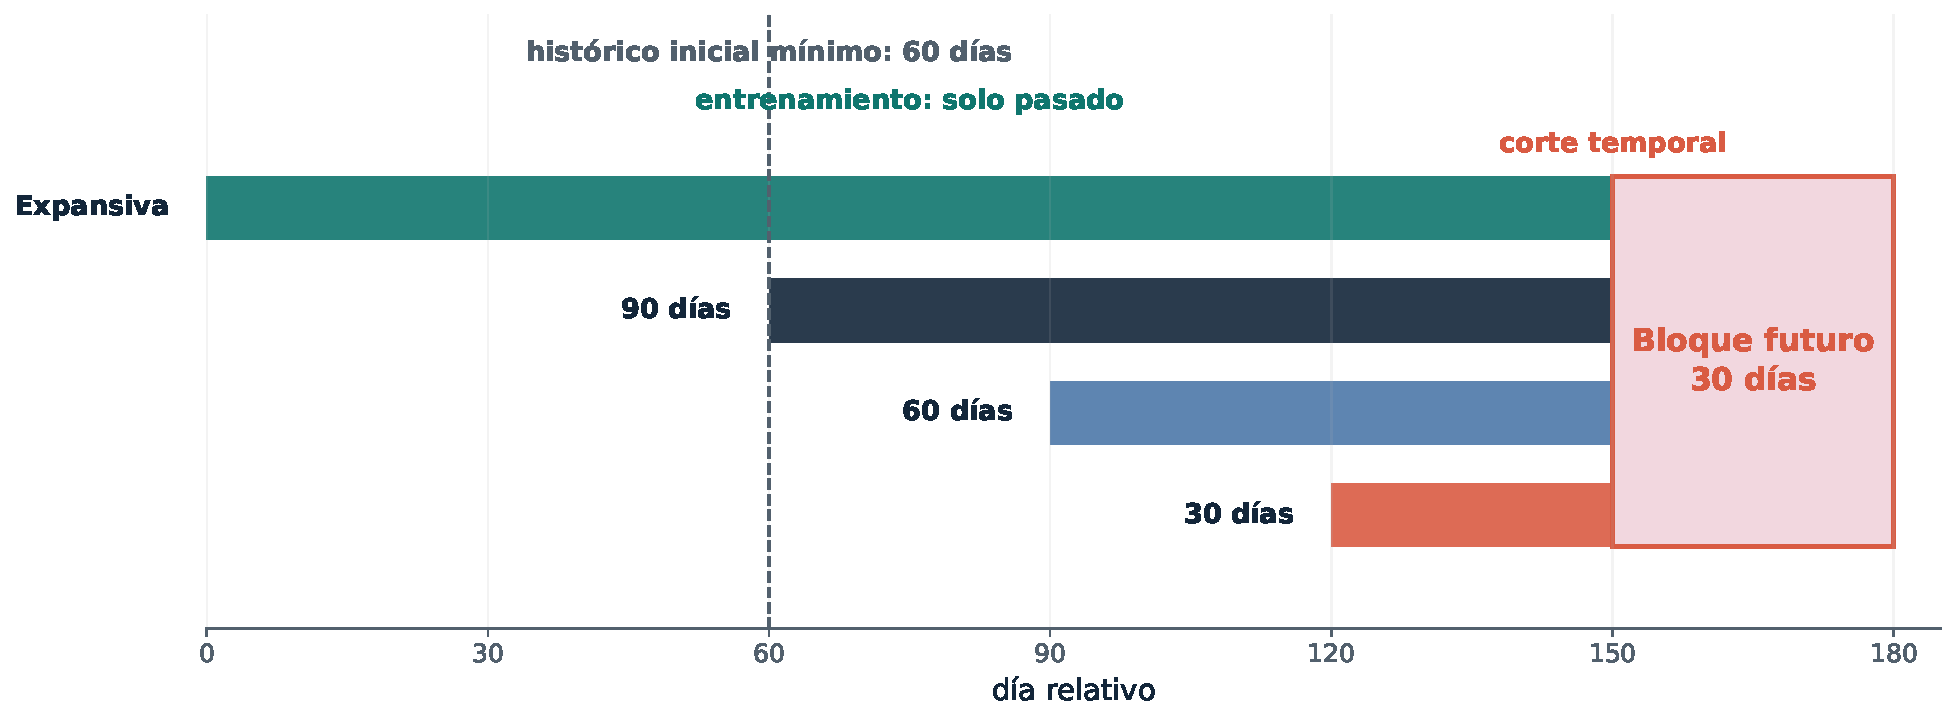
\includegraphics[width=0.94\textwidth]{protocolo_temporal.pdf}
  \end{center}
  \vspace{-0.15em}
  \begin{block}{Regla de actualización}
    \small PSI $>0,20$ \textbf{o} caída de AUC/recall/F1/costo $\rightarrow$ revisar la ventana y reentrenar. Sin alarma, conservar el modelo y continuar midiendo.
  \end{block}
\end{frame}

% 8 --------------------------------------------------------------------------
\begin{frame}{No existe una ventana dominante}
  \framesubtitle{Corrida canónica: \texttt{results/adaptive\_results.csv} · 4 bloques · XGBoost 180 árboles}
  \begin{columns}[T]
    \begin{column}{0.66\textwidth}
      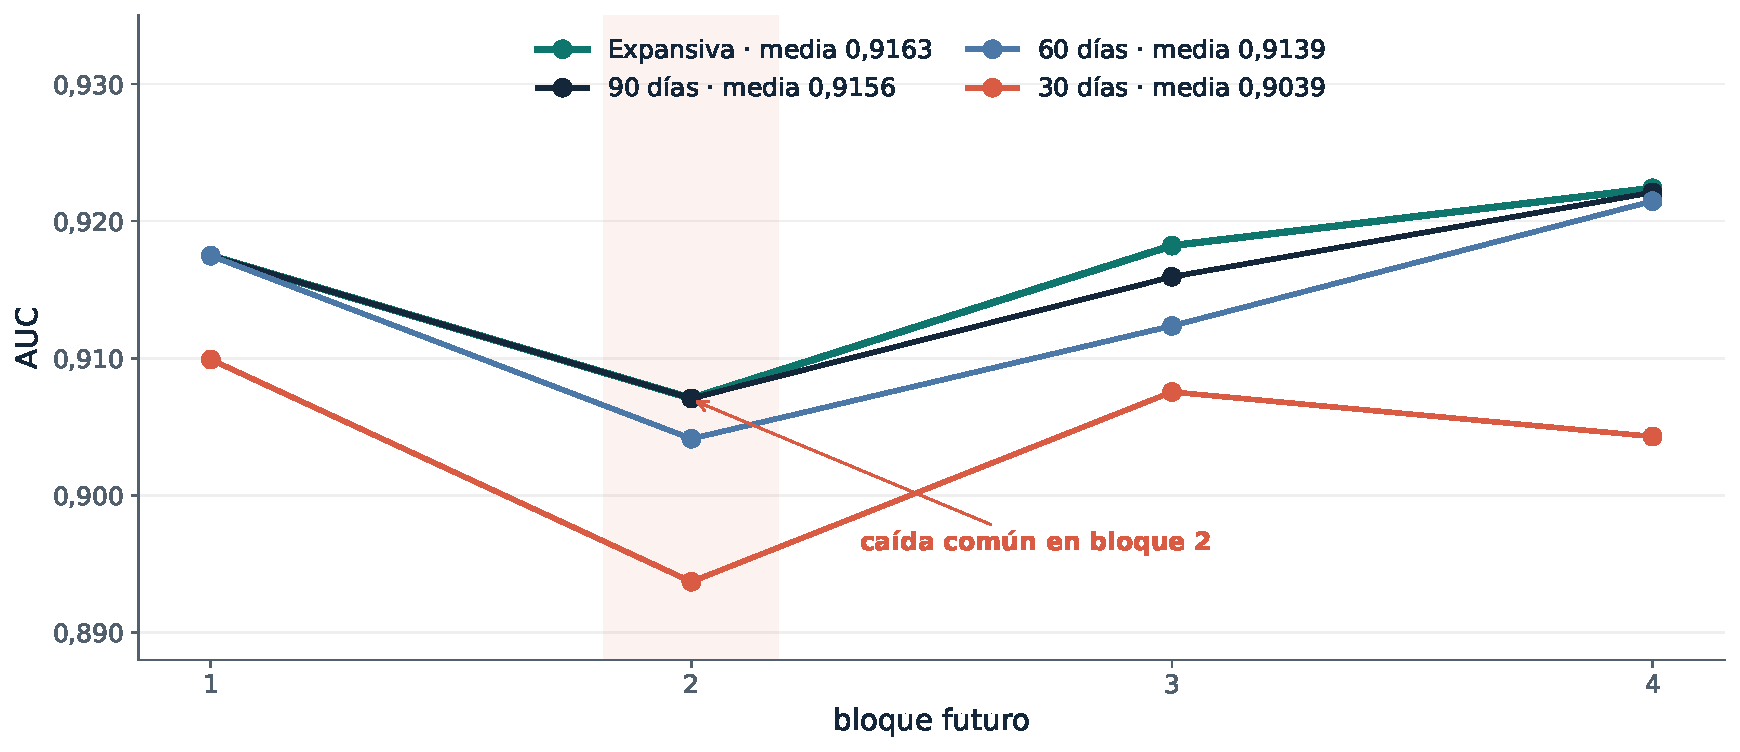
\includegraphics[width=\textwidth]{auc_adaptativo.pdf}
    \end{column}
    \begin{column}{0.32\textwidth}
      \begin{block}{Promedio por ventana}
        \scriptsize
        \setlength{\tabcolsep}{3pt}
        \begin{tabular}{@{}lrrr@{}}
          \toprule
          Ventana & AUC & F1 & Costo\\
          \midrule
          Expansiva & \textbf{0,9163} & 0,5575 & 17\,435\\
          90 días & 0,9156 & \textbf{0,5635} & \textbf{17\,336}\\
          60 días & 0,9139 & 0,5585 & 17\,635\\
          30 días & 0,9039 & 0,5481 & 18\,416\\
          \bottomrule
        \end{tabular}
      \end{block}
      \begin{alertblock}{Lectura correcta}
        \small Expansiva gana en AUC; 90 días gana en F1 y costo. El PSI medio máximo permanece bajo 0,05: monitorear solo drift no basta.
      \end{alertblock}
    \end{column}
  \end{columns}
\end{frame}

% 9 --------------------------------------------------------------------------
\begin{frame}{Recomendación operativa}
  \framesubtitle{La política depende del objetivo de decisión, no de una única métrica}
  \vspace{0.25em}
  \begin{center}
    \colorbox{mist}{\parbox{0.90\textwidth}{\centering
      \color{ink}\Large\bfseries Magic UID causal + ventana seleccionada por objetivo + umbral calibrado por costo}}
  \end{center}
  \vspace{0.55em}
  \begin{columns}[T]
    \begin{column}{0.31\textwidth}
      \begin{block}{Representación}
        \small Usar agregaciones por pseudo-cliente: aportaron \textbf{+0,0116} holdout y \textbf{+0,0162} OOF.
      \end{block}
    \end{column}
    \begin{column}{0.31\textwidth}
      \begin{block}{Ventana}
        \small \textbf{Expansiva} si se prioriza AUC; \textbf{90 días} si se prioriza F1 y costo.
      \end{block}
    \end{column}
    \begin{column}{0.31\textwidth}
      \begin{block}{Decisión}
        \small Iniciar en umbral \textbf{0,19}; monitorear recall, F1, AUC, PSI y costo por bloque.
      \end{block}
    \end{column}
  \end{columns}
  \vspace{0.55em}
  \begin{alertblock}{Siguiente paso}
    \centering Validar la política con costos reales de falso positivo/falso negativo y un bloque externo posterior.
  \end{alertblock}
\end{frame}

% 10 -------------------------------------------------------------------------
\appendix
\begin{frame}{Apéndice · reproducibilidad}
  \framesubtitle{Semillas, fuentes de datos y artefactos ejecutables}
  \begin{columns}[T]
    \begin{column}{0.47\textwidth}
      \begin{block}{Semillas}
        \small
        \begin{tabular}{@{}lr@{}}
          \toprule
          Notebook / script & Semilla\\
          \midrule
          01 baseline CPU & 0 (default)\\
          02 XGBoost GPU & 2019\\
          03 LightGBM & 47 / 11\\
          04 magic UID & sin semilla explícita\\
          05 integrado & \textbf{42}\\
          adaptativo & \textbf{42}\\
          \bottomrule
        \end{tabular}
      \end{block}
      \begin{block}{Hardware}
        \small 16 núcleos CPU · NVIDIA RTX 2060 6 GB · ejecución local sin submissions.
      \end{block}
    \end{column}
    \begin{column}{0.49\textwidth}
      \begin{block}{Fuentes canónicas}
        \scriptsize
        \texttt{results/RANKING\_FINAL.csv}\\
        \texttt{results/bench\_05\_integrated.csv}\\
        \texttt{results/threshold\_metrics\_xgb96.csv}\\
        \texttt{results/adaptive\_results.csv}
      \end{block}
      \begin{block}{Código y entregables}
        \scriptsize
        \texttt{codigos/ejecutados/01--05}\\
        \texttt{src/adaptive\_fraud.py}\\
        \texttt{presentacion/generar\_figuras.py}\\
        \texttt{informe\_latex/main\_entrega.pdf}
      \end{block}
    \end{column}
  \end{columns}
\end{frame}

\end{document}
